\documentclass[english, authoryear, preprint]{elsarticle}
\usepackage{booktabs}
\usepackage{multicol}
\usepackage{longtable}
\usepackage{dblfloatfix}
\usepackage{apalike}
\usepackage{fixltx2e}
\usepackage{enumitem}
\usepackage{amsmath}
\usepackage{float}
\renewcommand{\dblfloatpagefraction}{2.0}
\usepackage{array}
\newcolumntype{R}[1]{>{\raggedleft\let\newline\\\arraybackslash\hspace{0pt}}m{#1}}
\usepackage{balance}

\newcommand\bibsection{%
  \section*{\bibname\markright{\MakeUppercase{\bibname}}}}

\begin{document}
\begin{frontmatter}
\title{A Cross-Benchmark Comparison of 87 Learning to Rank Methods}
\author[avanade,ut]{Niek Tax\corref{cor}\fnref{fn}}
\ead{niek.tax@avanade.com}
\author[avanade]{Sander Bockting}
\ead{sander.bockting@avanade.com}
\author[ut]{Djoerd Hiemstra}
\ead{d.hiemstra@utwente.nl}
\cortext[cor]{Corresponding Author: Niek Tax, Avanade Netherlands B.V., Versterkerstraat 6,
1322AP Almere, the Netherlands; Email, niek.tax@avanade.com; Phone, +31634085760}
\fntext[fn]{Author is affiliated with the University of Twente, but this paper was written during his stay at Avanade Netherlands B.V.}
\address[avanade]{Avanade Netherlands B.V., Versterkerstraat 6,
1322AP Almere, the Netherlands}
\address[ut]{University of Twente, P.O. Box 217, 7500AE Enschede,
the Netherlands}
\begin{abstract}
Learning to rank is an increasingly important scientific field that comprises the use of machine learning for the ranking task. New learning to rank methods are generally evaluated on benchmark test collections. However, comparison of learning to rank methods based on evaluation results is hindered by non-existence of a standard set of evaluation benchmark collections. In this paper we propose a way to compare learning to rank methods based on a sparse set of evaluation results on a set of benchmark datasets. Our comparison methodology consists of two components: 1) Normalized Winning Number, which gives insight in the ranking accuracy of the learning to rank method, and 2) Ideal Winning Number, which gives insight in the degree of certainty concerning its ranking accuracy. Evaluation results of 87 learning to rank methods on 20 well-known benchmark datasets are collected through a structured literature search. ListNet, SmoothRank, FenchelRank, FSMRank, LRUF and LARF are the best performing learning to rank methods in increasing order of Normalized Winning Number and decreasing order of Ideal Winning Number.
\end{abstract}
\begin{keyword}
Learning to rank \sep Information retrieval \sep Evaluation metric
\end{keyword}
\end{frontmatter}

\section{Introduction}
Ranking is a core problem in the field of information retrieval. The ranking task in information retrieval entails the ranking of candidate documents according to their relevance to a given query. Ranking has become a vital part of web search, where commercial search engines help users find their need in the extremely large collection of the World Wide Web. Among useful applications outside web search are automatic text summarisation, machine translation, drug discovery and determining the ideal order of maintenance operations \citep{Rudin2009}. In addition, \cite{McNee2006} found the ranking task to be a better fit for recommender systems than the regression task (continuous scale predictions), which is currently still frequently used within such systems.\\

Research in the field of ranking models has been based on manually designed ranking functions, such as the well-known BM25 model \citep{Robertson1994}. Increased amounts of potential training data have recently made it possible to leverage machine learning methods to obtain more effective ranking models. Learning to rank is the relatively new research area that covers the use of machine learning models for the ranking task.\\

In recent years, several learning to rank benchmark datasets have been proposed with the aim of enabling comparison of learning to rank methods in terms of ranking accuracy. Well-known benchmark datasets in the learning to rank field include the \emph{Yahoo! Learning to Rank Challenge} datasets \citep{Chapelle2011a}, the \emph{Yandex Internet Mathematics 2009} contest\footnote{http://imat2009.yandex.ru/en}, the LETOR datasets \citep{Qin2010}, and the MSLR (Microsoft Learning to Rank) datasets\footnote{http://research.microsoft.com/en-us/projects/mslr/}. There exists no agreement among authors in the learning to rank field on the benchmark collection(s) to use to evaluate a new model. Comparing ranking accuracy of learning to rank methods is largely hindered by this lack of a standard way of benchmarking.\\

\cite{Gomes2013} analyzed the ranking accuracy of a set of models on both LETOR 3.0 and 4.0. \cite{Busa-Fekete2013} compared the accuracy of a small set of models over the LETOR 4.0 datasets, both MSLR datasets, both the Yahoo! Learning to Rank Challenge datasets and one of the datasets from LETOR 3.0. Both studies did not aim to be complete in benchmark datasets and learning to rank methods included in their comparisons. To our knowledge, no structured meta-analysis on ranking accuracy has been conducted where evaluation results on several benchmark collections are taken into account. In this paper we will perform a meta-analysis with the aim of comparing the ranking accuracy of learning to rank methods. The paper will describe two stages in the meta-analysis process: 1) collection of evaluation results, and 2) comparison of learning to rank methods.

\section{Collecting Evaluation Results}
\label{sec:collecting_evaluation_results}
We collect evaluation results on the datasets of benchmark collections through a structured literature search. Table \ref{tbl:ltr_benchmark_collections} presents an overview of the benchmark collections included in the meta-analysis.

\begin{table}[!h]
\centering
\begin{tabular}{p{8cm}R{3cm}}\toprule
Benchmark collection & \# of datasets \\
\midrule
AOL		  & 1\\
LETOR 2.0 & 3\\
LETOR 3.0 & 7\\
LETOR 4.0 & 2\\
MSLR	  & 2\\
WCL2R	  & 2\\
Yahoo! Learning to Rank Challenge 	     & 2\\
Yandex Internet Mathematics 2009 contest & 1\\
\textbf{Total} & \textbf{20}\\ 	
\bottomrule
\end{tabular}
\caption{Included learning to rank evaluation benchmark collections}
\label{tbl:ltr_benchmark_collections}
\end{table}

For the LETOR collections, the evaluation results of the baseline models will be used from LETOR 2.0\footnote{http://research.microsoft.com/en-us/um/beijing/projects/letor/letor2.0/baseline.aspx}, 3.0\footnote{http://research.microsoft.com/en-us/um/beijing/projects/letor/letor3baseline.aspx} and 4.0\footnote{http://research.microsoft.com/en-us/um/beijing/projects/letor/letor4baseline.aspx} as listed on the LETOR website.\\

LETOR 1.0 and 3.0, Yahoo! Learning to Rank Challenge, WCL2R and AOL have accompanying papers that were released with the collection. Authors publishing evaluation results on these benchmark collections are requested to cite these papers. We collect evaluation measurements of learning to rank methods on these benchmark collections through forward literature search. Table~\ref{tbl:ltr_benchmark_forref} presents an overview of the results of this forward literature search performed using Google Scholar.\\
\begin{table}[!h]
\centering
\begin{tabular}{p{6cm}p{3cm}R{2cm}}\toprule
Benchmark & Paper & \# of forward references \\
\midrule
LETOR 1.0 \& 2.0 & \cite{Liu2007b} & 307\\
LETOR 3.0 & \cite{Qin2010} & 105\\
Yahoo! Learning to Rank Challenge & \cite{Chapelle2011a} & 102\\
AOL dataset & \cite{Pass2006} & 339\\
WCL2R & \cite{Alcantara2010} & 2\\
\bottomrule
\end{tabular}
\caption{Forward references of learning to rank benchmark papers}
\label{tbl:ltr_benchmark_forref}
\end{table}

The LETOR 4.0, MSLR-web10/30k and Yandex Internet Mathematics Competition 2009 benchmark collections are not accompanied by a paper. To collect evaluation results for learning to rank methods on these benchmarks, a Google Scholar search is performed on the name of the benchmark. Table~\ref{tbl:ltr_benchmark_searches} shows the results of this literature search.

\begin{table}[!h]
\centering
\begin{tabular}{p{8cm}R{3cm}}\toprule
Search Query & Google scholar search results \\
\midrule
"LETOR 4.0" & 75 \\
"MSLR-web10k" & 16 \\
"MSLR-web30k" & 15 \\
"Yandex Internet Mathematics" & 3\\
\bottomrule
\end{tabular}
\caption{Google scholar search results for learning to rank benchmarks}
\label{tbl:ltr_benchmark_searches}
\end{table}

\subsection{Literature Selection}
Table \ref{tab:ltr_methods_used} in the appendix gives an overview of the learning to rank methods for which evaluation results were found through the described procedure. Occurrences of L2, L3 and L4 in Table \ref{tab:ltr_methods_used} imply that these algorithms are evaluated as official LETOR 2.0, 3.0 and 4.0 baselines respectively.\\

Some studies with evaluation results found through the literature search procedure were not usable for the meta-analysis. The following enumeration enumerates those properties that made one or more studies unusable for the meta-analysis. Between brackets are the studies that these properties apply to.

\begin{enumerate}[noitemsep,nolistsep]
\item A different evaluation methodology was used in the study compared to what was used in other studies using the same benchmark \citep{Geng2011, Lin2012}
\item The study focuses on a different learning to rank task (e.g. rank aggregation or transfer ranking) \citep{De2011, De2010, Derhami2013, De2012, Chen2010, Ah-Pine2008, Wang2009c, De2013, Miao2013, Hoi2008, De2012b, Duh2011b, Argentini2012, Qin2010c, Volkovs2013, Desarkar2011, Pan2013, Lin2011b, Volkovs2012, Dammak2011}
\item The study used an altered version of a benchmark that contained additional features \citep{Bidoki2009, Ding2010}
\item The study provides no exact data of the evaluation results (e.g. results are only in graphical form) \citep{Wang2008, Wang2010, Xu2010, Kuo2009, Li2008, Xia2008, Zhou2011, Wu2011, Zhu2009, Karimzadehgan2011, Swersky2012, Pan2011, Ni2008, Ciaramita2008, Stewart2012, Petterson2009, Agarwal2010, Chang2009, Qin2008c, Adams2011, Sculley2009, Huang2008, Alejo2010, Sun2011, He2010b, Benbouzid2012, Geng2012, Chen2012, Xu2012, Shivaswamy2011}
\item The study reported evaluation results in a different metric than the metrics chosen for this meta-analysis \citep{Yu2009, Thuy2009, Pahikkala2009, Kersting2009, Mohan2011}
\item The study reported a higher performance on baseline methods than official benchmark runs \citep{Dubey2009, Banerjee2009, Peng2010b, Song2014, Bian2010, Bian2010b, Carvalho2008, Acharyya2012, Peng2010b, Tran2012, Asadi2013c}
\item The study did not report any baseline performance that allowed us to check validity of the results \citep{Chakrabarti2008, Wang2012b, Buffoni2011}.
\end{enumerate}

\section{A Methodology for Comparing Learning to Rank Methods Cross-Benchmark}
\cite{Qin2010} state that it may differ between datasets what the most accurate ranking methods are. They propose a measure they call \emph{Winning Number} to evaluate the overall performance of learning to rank methods over the multiple datasets in the LETOR 3.0 collection. Winning Number is defined as the number of other algorithms that an algorithm can beat over the set of datasets, or more formally\\

$\text{WN}_i(M) = \sum\nolimits_{j=1}^n \sum\nolimits_{k=1}^m I_{\{M_i(j)>M_k(j)\}}$\\

where $j$ is the index of a dataset, $n$ the number of datasets in the comparison, $i$ and $k$ are indices of an algorithm, $M_i(j)$ is the performance of the $i$-th algorithm on the $j$-th dataset, $M$ is a ranking measure (such as NDCG or MAP), and $I_{\{M_i(j)>M_k(j)\}}$ is an indicator function such that\\

$I_{\{M_i(j)>M_k(j)\}} = \begin{cases}
1 & \text{if } M_i(j) > M_k(j), \\
0 & \text{otherwise}
\end{cases}$\\

The LETOR 3.0 was a comparison on a \emph{dense} set of evaluation results, in the sense that there were evaluation results available for all learning to rank algorithms on all datasets included in their comparison. The Winning Number evaluation metric relies on the denseness of the evaluation results set. In contrast to the LETOR 3.0 comparison, our set of evaluation results will be sparse. We propose a normalized version of the Winning Number metric to enable comparison of a sparse set of evaluation results. This Normalized Winning Number takes only those datasets into account that an algorithm is evaluated on and divides this by the theoretically highest Winning Number that an algorithm would have had in case it it would have been the most accurate algorithm on all datasets on which it has been evaluated. We will redefine the indicator function $I$ in order to only take into account those datasets that an algorithm is evaluated on, as\\

$I^{'}_{M_i(j)>M_k(j)} = \begin{cases}
1 & \parbox[t]{5cm}{if $M_i(j)$ and $M_k(j)$ are both defined and $M_i(j) > M_k(j)$,}\\
0 & \parbox[t]{5cm}{otherwise}
\end{cases}$\\

From now on this adjusted version of Winning Number will be references to as \emph{Normalized Winning Number (NWN)}. The mathematical definition of Normalized Winning Number is\\

$\text{NWN}_i(M) = \frac{\text{WN}_i(M)}{\text{IWN}_i(M)}$\\

\noindent
where $IWN$ is the Ideal Winning Number, defined as\\

$\text{IWN}_i(M) = \sum\nolimits_{j=1}^n \sum\nolimits_{k=1}^m D_{\{M_i(j),M_k(j)\}}$\\

where $j$ is the index of a dataset, $n$ the number of datasets in the comparison, $i$ and $k$ are indices of an algorithm, $M_i(j)$ is the performance of the $i$-th algorithm on the $j$-th dataset, $M$ is a ranking measure (such as NDCG or MAP), and $D_{\{M_i(j),M_k(j)\}}$ is an evaluation definition function such that\\

$D_{\{M_i(j),M_k(j)\}} = \begin{cases}
1 & \text{if } M_i(j) \text{ and } M_k(j) \text{ are both defined}, \\
0 & \text{otherwise}
\end{cases}$\\

NDCG@$\{3,5,10\}$ and MAP are the most frequently used evaluation metrics in the used benchmark collections combined, therefore we will limit our meta-analysis to evaluation results reported in one of these four metrics.

\section{Results of Learning to Rank Comparison}
The following subsections provide the performance of learning to rank methods in terms of NWN for NDCG@$\{3,5,10\}$ and MAP. Performance of the learning to rank methods is plotted with NWN on the vertical axis and the number of datasets on which the method has been evaluated on the horizontal axis. Moving to the right, certainty on the performance of the method increases. The methods for which it holds that there is no other method that has 1) a higher NWN and 2) a higher number datasets evaluated, are identified as the best performing methods and are labeled. Table \ref{tab:raw_data} in the appendix provides raw NWN data for the learning to rank methods at NDCG@$\{3,5,10\}$ and MAP and their cross-metric weighted average.

\subsection{NDCG@3}
\begin{figure}
\centering
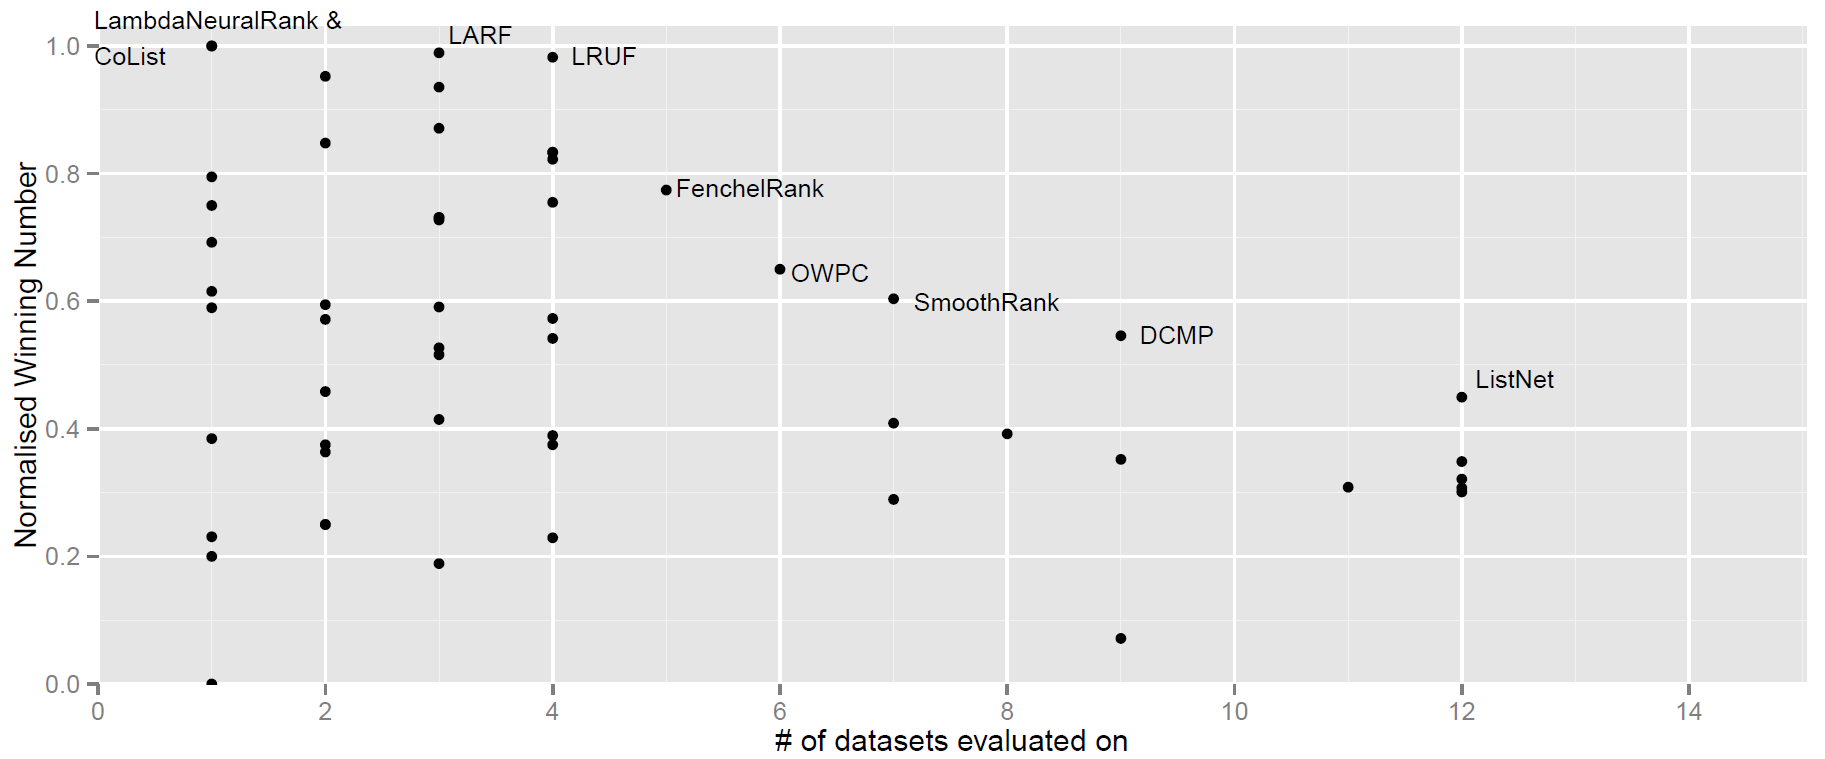
\includegraphics[scale=0.26]{gfx/ndcg3_winnum}
\caption{NDCG@3 comparison of 87 learning to rank methods}
\label{fig:normalized_winning_number_ndcg3}
\end{figure}
Figure \ref{fig:normalized_winning_number_ndcg3} shows the NWN of learning to rank methods based on NDCG@3 results. LambdaNeuralRank and CoList both acquired a NWN score of 1.0 by beating all other algorithms on one dataset, with LambdaNeuralRank winning on the AOL dataset and CoList winning on Yahoo Set 2. LARF and LRUF scored very high scores of near 1.0 on three of the LETOR 3.0 datasets, which results in more certainty on these methods' performance because they are validated on three datasets that additionally are more relevant than AOL and Yahoo Set 2 (number of evaluation results for LETOR 3.0 are higher than those for AOL and Yahoo set 2). FenchelRank, OWPC, SmoothRank, DCMP and ListNet are ordered decreasingly by NWN and at the same time increasingly in number of datasets that they are evaluated on, resulting in a higher degree of certainty on the accuracy of the algorithms.\\

LambdaNeuralRank, CoList, LARF, LRUF, OWPC and DCMP evaluation results are all based on one study, therefore are subjected to the risk of one overly optimistic study producing those results. FenchelRank evaluation result are based combined result from two studies, although those studies have overlap in authors. SmoothRank and ListNet have the most reliable evaluation result source, as they were official LETOR baseline runs.  

\subsection{NDCG@5}
\begin{figure}
\centering
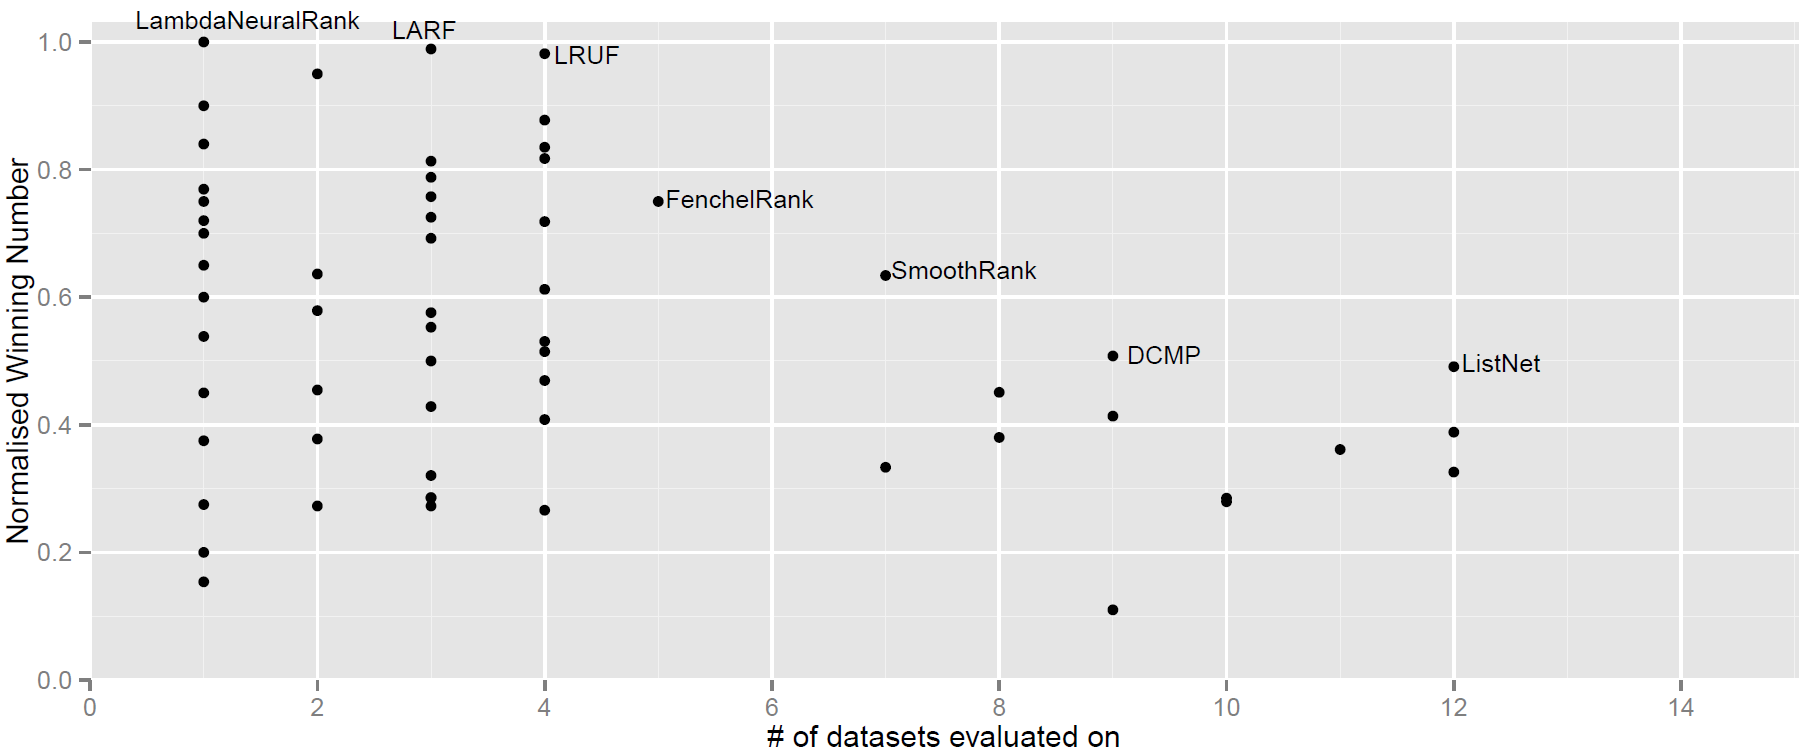
\includegraphics[scale=0.26]{gfx/ndcg5_winnum}
\caption{NDCG@5 comparison of 87 learning to rank methods}
\label{fig:normalized_winning_number_ndcg5}
\end{figure}
Figure \ref{fig:normalized_winning_number_ndcg5} shows the NWN of learning to rank methods based on NDCG@5 results. LambdaNeuralRank again beat all other methods solely with results on the AOL dataset scoring a NWN of 1.0. LARF, LRUF, FenchelRank, SmoothRank, DCMP and ListNet are from left to right evaluated on an increasing number of datasets, but score decreasingly well in terms of NWN. These results are highly in agreement with the NDCG@3 comparison. The only modification compared to the NDCG@3 comparison being that OWPC did show to be a method for which there were no methods performing better on both axes in the NDCG@5 comparison, but not in the @3 comparison. Like in the NDCG@3 comparison, SmoothRank and ListNet can be regarded as most reliable results because the evaluation measurements for these methods are based on LETOR official baselines.

\subsection{NDCG@10}
\begin{figure}
\centering
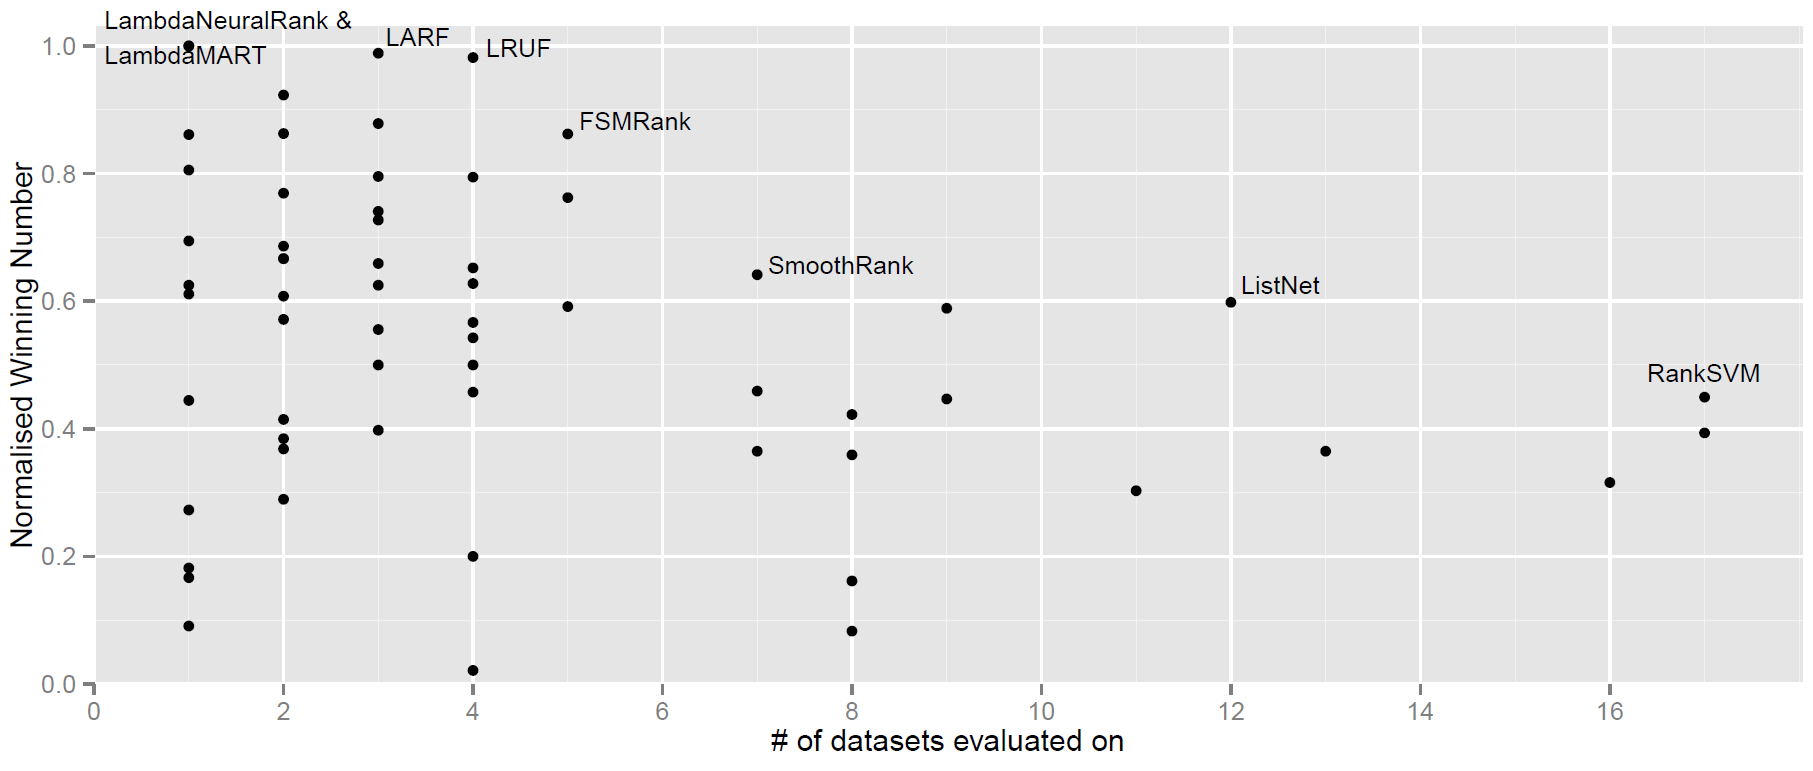
\includegraphics[scale=0.26]{gfx/ndcg10_winnum}
\caption{NDCG@10 comparison of 87 learning to rank methods}
\label{fig:normalized_winning_number_ndcg10}
\end{figure}

Figure \ref{fig:normalized_winning_number_ndcg10} shows the NWN of learning to rank methods based on NDCG@10 results. LambdaMART and LambdaNeuralRank score a NWN of 1.0 on the NDCG@10 comparison. For LambdaNeuralRank these results are again based on AOL dataset measurements. LambdaMART showed the highest NDCG@10 performance for the MSLR-WEB10k dataset. The set of algorithms for which there is no other algorithm with both a higher NWN and number of datasets evaluated on is partly in agreement with those for the NDCG@3 and @5 comparisons: {LARF, LRUF, FSMRank, SmoothRank, ListNet, RankSVM}. In contrast to the NDCG@3 and @5 comparison, DCMP is not among the best algorithms.

\subsection{MAP}
\begin{figure}
\centering
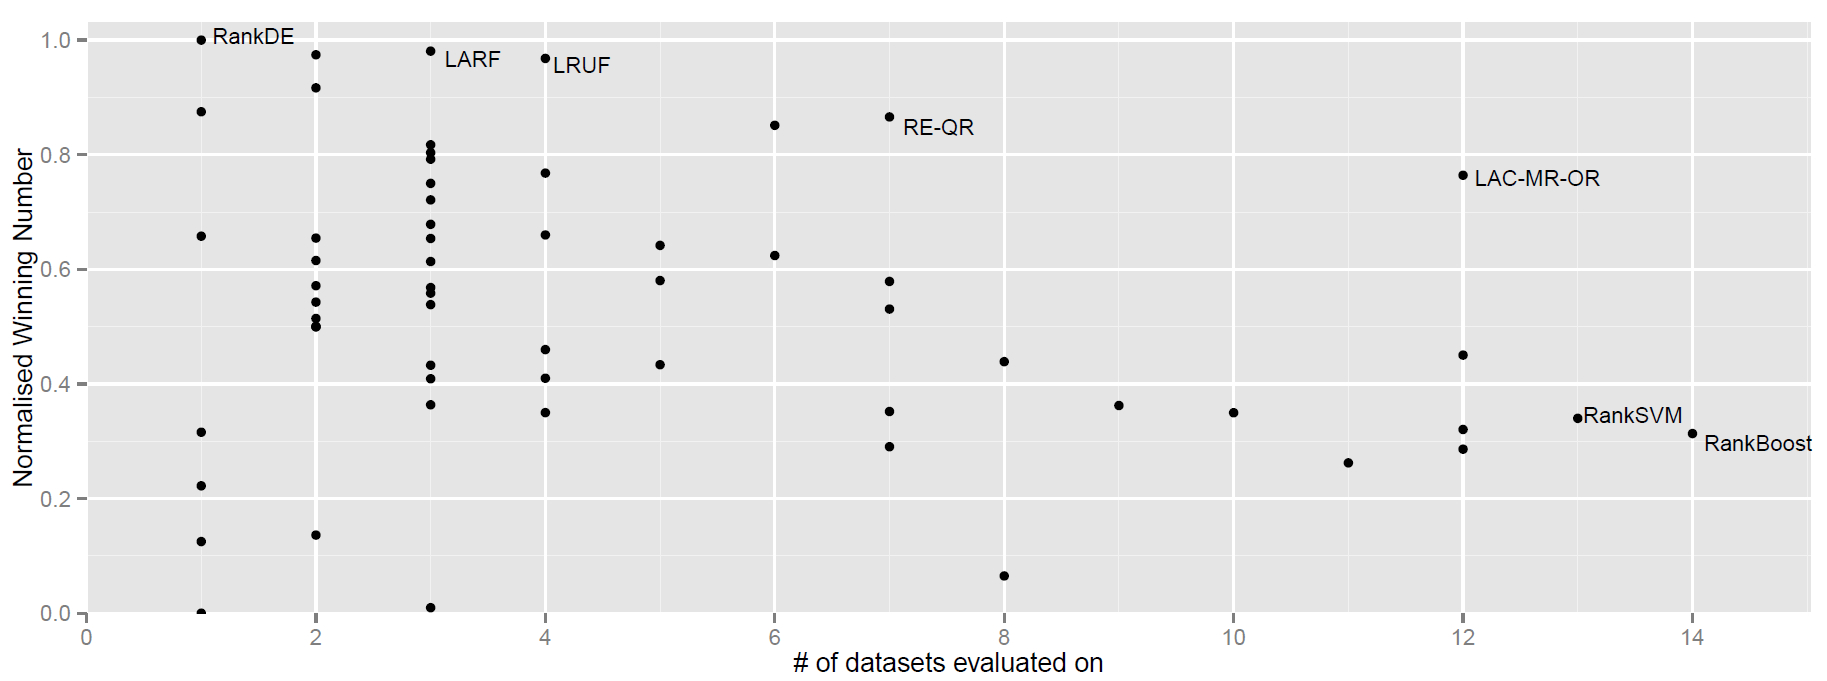
\includegraphics[scale=0.26]{gfx/map_winnum}
\caption{MAP comparison of 87 learning to rank methods}
\label{fig:normalized_winning_number_map}
\end{figure}
Figure \ref{fig:normalized_winning_number_map} shows the NWN of learning to rank methods based on MAP results. Comparisons on the NDCG metrics where highly in agreement on the best performing algorithms, MAP-based NWN results show different results. RankDE scores a NWN of 1.0 on one dataset, which is achieved by obtaining highest MAP-score on the LETOR 2.0 TD2003 which has many evaluation results are evaluated.\\

LARF and LRUF score very high NWN scores, but based on only few datasets, just as in the NDCG-based comparisons. Notable is that low performance of SmoothRank and ListNet, given that those methods were top performing methods in the NDCG-based comparisons. Table \ref{tab:raw_data} in the appendix shows that LAC-MR-OR is evaluated on more datasets on MAP than on NDCG, thereby LAC-MR-OR obtained equal certainty to ListNet with a higher NWN. SmoothRank performed a NWN of around 0.53 over 7 datasets, which is still good in both certainty and accuracy, but not among the top methods. RE-QR is one of the best performers in the MAP comparison with a reasonable amount of benchmark evaluations. No reported NDCG performance was found in the literature search for RE-QR. There is a lot of certainty on the accuracy of RankBoost and RankSVM as both models are evaluated on the majority of datasets included in the comparison for the MAP metric, but given their NWN it can said that both methods are not within the top performing learning to rank methods.

\subsection{Cross-Metric}
\begin{figure}
\centering
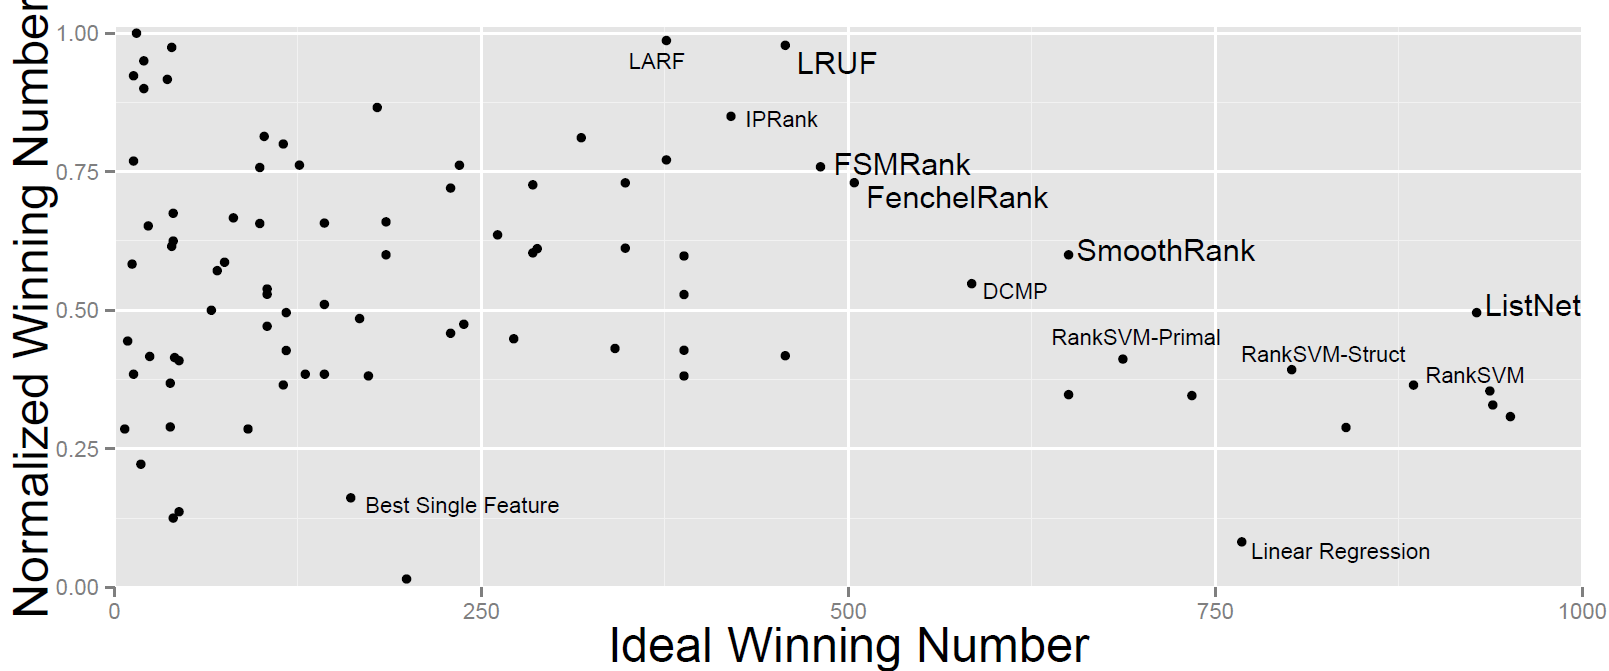
\includegraphics[scale=0.28]{gfx/combined_normalized_winnum}
\caption{Cross-benchmark comparison of 87 learning to rank methods}
\label{fig:normalized_winning_number_all}
\end{figure}
Figure \ref{fig:normalized_winning_number_all} shows the NWN as function of IWN for the methods described in Table \ref{tab:ltr_methods_used}. The cross-metric comparison is based on the NDCG@$\{3,5,10\}$ and MAP comparisons combined, which justifies analysing the comparison more thoroughly. Figure \ref{fig:normalized_winning_number_all} labels the algorithms with no other algorithm having a higher value on both the horizontal axis and vertical axis, but also labels the algorithms with exactly one algorithm having a higher value on both axes with smaller font size. In addition, Linear Regression and the ranking method of simply sorting on the best single feature are labelled as baselines.\\

LRUF, FSMRank, FenchelRank, SmoothRank and ListNet showed to be the methods that have no other method superior to them in both IWN and NWN. LRUF is the only method that achieved this in all NDCG comparisons, the MAP comparison as well as the cross-metric comparison. With FenchelRank, FSMRank, SmoothRank and ListNet being among the top performing methods in all NDCG comparisons as well as in the cross-metric comparison, it can be concluded that the cross-metric results are highly defined by the NDCG performance as opposed to the MAP performance. This was to be expected, because the cross-metric comparison input data of three NDCG entries (@3, @5, and @10) enables it to have up to three times as many as many weight as the MAP comparison.\\

LARF, IPRank and DCMP and several variants of RankSVM performed very well on the cross-metric comparison, with all having only one method in its top right quadrant. LARF also performed among the top methods on the NDCG and MAP comparisons and DCMP was a top performer in a few of the NDCG comparisons. C-CRF, DirectRank, FP-Rank, RankCSA, LambdaNeuralRank and VFLR all have a near-perfect NWN value, but have a low IWN value. Further evaluation runs of these methods on benchmark datasets that they are not yet evaluated on are desirable. The DirectRank paper \cite{Tan2013} shows that the method  is evaluated on more datasets than the number of datasets that we included evaluation results for in this meta-analysis. Some of the DirectRank measurements could not be used because measurements on some datasets were only available in graphical form and not in raw data.\\

LAC-MR-OR and RE-QR showed very good ranking accuracy in the MAP comparison on multiple datasets. Because LAC-MR-OR is only evaluated on two datasets for NDCG@10 and RE-QR is not evaluated for NDCG at all, LAC-MR-OR and RE-QR are not within the top performing methods in the cross-metric comparison. 

\section{Limitations}
In the NWN calculation, the weight of each benchmark on the total score is determined by the number of evaluation measurements on this benchmark. By calculating it in this way, we implicitly make the assumption that the learning to rank methods are (approximately) distributed uniformly over the benchmarks, such that the average learning to rank method tested are approximately equally hard for each data set. It could be the case however that this assumption is false and that the accurateness of the learning to rank methods on a dataset is not dataset independent.\\

A second limitation is that the datasets on which learning to rank methods have been evaluated cannot always be regarded a random choice. It might be the case that some researchers chose to publish results for exactly those benchmark datasets that showed the most positive results for their learning to rank method.\\

Another limitation is that our comparison methodology relies on the correctness of the evaluation results found in the literature search step. This brings up a risk of overly optimistic evaluation results affecting our NWN results. Limiting the meta-analysis to those studies that report comparable results on one of the baseline methods of a benchmark set reduces this limitation but does not solve it completely. By taking IWN into account in Figure \ref{fig:normalized_winning_number_all} we further mitigate this limitation, as IWN is loosely related with the number of studies that reported evaluation results for an algorithm.\\

Our comparison regarded evaluation results on NDCG@$\{3,5,10\}$ and MAP. By making the decision to include NDCG at three cut-off points and only a single MAP entry, we implicitly attain a higher weight for NDCG compared to MAP on an analysis that combines all measurements on the four metrics. This implicit weighting could be regarded as arbitrary, but the number of algorithm evaluation results gained by this makes it a pragmatic approach. Note that another implicit weighting lies in the paper dimension. Hence, the higher number of evaluation results specified in a paper, the higher the influence of this paper on the outcome of the analysis. This implicit weighting is not harmful to the validity of our comparison, as papers with a large number of evaluation results are more valuable than papers with a few evaluation results. In addition, papers with a high number of evaluation results are not expected to be less reliable than papers with fewer evaluation results.

\section{Contributions}
We proposed a new way of comparing learning to rank methods based on sparse evaluation results data on a set of benchmark datasets. Our comparison methodology comprises of two components: 1) NWN, which provides insight in the ranking accuracy of the learning to rank method, and 2) IWN, which gives insight in the degree of certainty concerning the performance of the ranking accuracy.\\

Based on our literature search for evaluation results on well-known benchmarks collections, a lot of insight has been gained with the cross-benchmark comparison on which methods tend to perform better than others. However, no closing arguments can be formulated on which learning to rank methods are most accurate. LRUF, FSMRank, FenchelRank, SmoothRank and ListNet were the learning to rank algorithms for which it holds that no other algorithm produced more accurate rankings with a higher degree of certainty of ranking accuracy. From left to right, the ranking accuracy of these methods decreases while the certainty of the ranking accuracy increases.\\

More evaluation runs are needed for the methods on the left side of Figure \ref{fig:normalized_winning_number_all}. Our work contributes to this by identifying promising learning to rank methods that researchers could focus on in performing additional evaluation runs.

\bibliographystyle{apalike}
\bibliography{Bibliography}
\newpage
\appendix
\section{Meta-analysis Ranking Methods \& Data Sources}

{\fontsize{5.5pt}{5.4pt}\selectfont
\begin{longtable}{p{2.671cm}p{2.812cm}p{7.7cm}}\toprule
Method & Described in & Evaluated in\\
\midrule
AdaRank-MAP & \cite{Xu2007} & L2, L3, L4 \\
AdaRank-NDCG & \cite{Xu2007} & L2, L3, L4,  \cite{Busa-Fekete2013,Tan2013} \\ 
ADMM & \cite{Duh2011} & \cite{Duh2011} \\ 
ApproxAP & \cite{Qin2010b} & \cite{Qin2010b} \\ 
ApproxNDCG & \cite{Qin2010b} & \cite{Qin2010b} \\ 
BagBoo & \cite{Pavlov2010} & \cite{Ganjisaffar2011c} \\ 
Best Single Feature &  & \cite{Gomes2013} \\ 
BL-MART & \cite{Ganjisaffar2011c} & \cite{Ganjisaffar2011c} \\ 
BoltzRank-Single & \cite{Volkovs2009} & \cite{Volkovs2009, Volkovs2013} \\ 
BoltzRank-Pair & \cite{Volkovs2009} & \cite{Volkovs2009, Ganjisaffar2011c, Volkovs2013} \\ 
BT & \cite{Zhou2008} & \cite{Zhou2008} \\ 
C-CRF & \cite{Qin2008b} & \cite{Qin2008b} \\ 
CA & \cite{Metzler2007} & \cite{Busa-Fekete2013,Tan2013} \\ 
CCRank & \cite{Wang2011c} & \cite{Wang2011c} \\ 
CoList & \cite{Gao2014} & \cite{Gao2014} \\
Consistent-RankCosine & \cite{Ravikumar2011} & \cite{Tan2013} \\
DCMP & \cite{Renjifo2012}  & \cite{Renjifo2012}  \\
DirectRank & \cite{Tan2013} & \cite{Tan2013} \\
EnergyNDCG & \cite{Freno2011} & \cite{Freno2011} \\
FBPCRank & \cite{Lai2011} & \cite{Lai2011} \\
FenchelRank & \cite{Lai2013} & \cite{Lai2013, Lai2013b, Laporte2013} \\ 
FocusedBoost & \cite{Niu2012} & \cite{Niu2012} \\ 
FocusedNet & \cite{Niu2012} & \cite{Niu2012} \\ 
FocusedSVM & \cite{Niu2012} & \cite{Niu2012} \\ 
FP-Rank & \cite{Song2013} & \cite{Song2013} \\ 
FRank & \cite{Tsai2007} & L2, L3, \cite{Wang2012} \\ 
FSMRank & \cite{Lai2013c} & \cite{Lai2013c,Laporte2013} \\ 
FSM$^{SVM}$ & \cite{Lai2013c} & \cite{Lai2013c} \\
GAS-E & \cite{Geng2007} & \cite{Lai2013c} \\ 
GP & \cite{DeAlmeida2007} & \cite{Alcantara2010} \\
GPRank & \cite{Silva2009} & \cite{Torkestani2012} \\  
GRankRLS & \cite{Pahikkala2010} & \cite{Pahikkala2010} \\
GroupCE & \cite{Lin2011} & \cite{Lin2011} \\ 
GroupMLE & \cite{Lin2010} & \cite{Lin2011} \\ 
IntervalRank & \cite{Moon2010} & \cite{Moon2010, Freno2011} \\
IPRank & \cite{Wang2009b} & \cite{Wang2009b, Torkestani2012} \\ 
KeepRank & \cite{Chen2009} & \cite{Chen2009} \\
KL-CRF & \cite{Volkovs2011} & \cite{Volkovs2011} \\ 
LAC-MR-OR & \cite{Veloso2008} & \cite{Veloso2008, Alcantara2010} \\ 
LambdaMART & \cite{Burges2010} & \cite{Asadi2013a, Ganjisaffar2011c} \\ 
LambdaNeuralRank & \cite{Papini2012} & \cite{Papini2012} \\ 
LambdaRank & \cite{Burges2006} & \cite{Papini2012, Tan2013} \\ 
LARF & \cite{Torkestani2012} & \cite{Torkestani2012} \\
Linear Regression & \cite{Cossock2006} & L3, \cite{Wang2012, Volkovs2011} \\
ListMLE & \cite{Xia2008} & \cite{Lin2010, Lin2011, Gao2014} \\
ListNet & \cite{Cao2007} & L2, L3, L4 \\
ListReg & \cite{Wu2011} & \cite{Wu2011}\\
LRUF & \cite{Torkestani2012b} & \cite{Torkestani2012b}\\
MCP & \cite{Laporte2013} & \cite{Laporte2013}\\
MHR & \cite{Qin2007} & L2\\
MultiStageBoost & \cite{Kao2013} & \cite{Kao2013}\\
NewLoss & \cite{Peng2010} & \cite{Peng2010}\\
OWPC & \cite{Usunier2009} & \cite{Usunier2009}\\
PERF-MAP & \cite{Pan2011} & \cite{Torkestani2012b}\\
PermuRank & \cite{Xu2008} & \cite{Xu2008}\\
Q.D.KNN & \cite{Geng2008} & \cite{Wang2013}\\
RandomForest & \cite{Gomes2013} & \cite{Gomes2013}\\
Rank-PMBGP & \cite{Sato2013} & \cite{Sato2013}\\
RankAggNDCG & \cite{Wang2013} & \cite{Wang2013}\\
RankBoost & \cite{Freund2003} & L2, L3, L4, \cite{Busa-Fekete2013, Alcantara2010, Sato2013}\\
RankBoost (Kernel-PCA) & \cite{Duh2008} & \cite{Duh2008, Sato2013}\\
RankBoost (SVD) & \cite{Lin2009} & \cite{Lin2009}\\
RankCSA & \cite{He2010} & \cite{He2010}\\
RankDE & \cite{Bollegala2011} & \cite{Sato2013}\\
RankELM (pairwise) & \cite{Zong2013} & \cite{Zong2013}\\
RankELM (pointwise) & \cite{Zong2013} & \cite{Zong2013}\\
RankMGP & \cite{Lin2012} & \cite{Lin2012}\\
RankNet & \cite{Burges2005} & \cite{Busa-Fekete2013, Papini2012, Niu2012}\\
RankRLS & \cite{Pahikkala2009} & \cite{Pahikkala2010}\\
RankSVM & \cite{Herbrich1999, Joachims2002} & L2, L3, \cite{Busa-Fekete2013, Freno2011, He2010, Alcantara2010, Papini2012}\\
RankSVM-Struct &  & L3, L4\\
RankSVM-Primal &  & L3, \cite{Lai2011}\\
RCP & \cite{Elsas2008} & \cite{Elsas2008}\\
RE-QR & \cite{Veloso2010} & \cite{Veloso2010}\\
REG-SHF-SDCG & \cite{Wu2009} & \cite{Wu2009}\\
Ridge Regression & \cite{Cossock2006} & L3\\
RSRank & \cite{Sun2009} & \cite{Lai2013}\\
SmoothGrad & \cite{Le2007} & \cite{Tan2013}\\
SmoothRank & \cite{Chapelle2010} & L3, \cite{Chapelle2010}\\
SoftRank & \cite{Taylor2008, Guiver2008} & \cite{Qin2010b}\\
SortNet & \cite{Rigutini2008} & \cite{Rigutini2008,Freno2011, Papini2012}\\
SparseRank & \cite{Lai2013b} & \cite{Lai2013b}\\
SVM$^{MAP}$ & \cite{Yue2007} & L3, \cite{Wang2012, Xu2008, Niu2012}\\
SwarmRank & \cite{Diaz-Aviles2009} & \cite{Sato2013}\\
TGRank & \cite{Lai2013} & \cite{Lai2013}\\
TM & \cite{Zhou2008} & \cite{Zhou2008, Papini2012, Tan2013}\\
VFLR & \cite{Cai2012} & \cite{Cai2012}\\
\bottomrule
\caption{Learning to rank algorithms with measurements on benchmark datasets}
\label{tab:ltr_methods_used}
\end{longtable}
}

\newpage
\section{Meta-analysis Raw Data}
{\fontsize{5.5pt}{5.4pt}\selectfont
\begin{longtable}{@{}lrrrrrrrrrrrrrrrr@{}}\toprule
& \multicolumn{2}{c}{NDCG@3} & \phantom{a} 
& \multicolumn{2}{c}{NDCG@5} & \phantom{a} 
& \multicolumn{2}{c}{NDG@10} & \phantom{a} 
& \multicolumn{2}{c}{MAP}    & \phantom{a}
& \multicolumn{3}{c}{CROSS}\\
\cmidrule{2-3} \cmidrule{5-6} \cmidrule{8-9} \cmidrule{11-12} \cmidrule{14-16}
Method & NWN & \#ds && NWN & \#ds && NWN & \#ds && NWN & \#ds && WN & IWN & NWN \\ \midrule\endhead
AdaRank-MAP & 0.3529 & 12 && 0.3884 & 12 && 0.3648 & 13 && 0.3206 & 12 && 334 & 940 & 0.3553 \\
AdaRank-NDCG & 0.3122 & 12 && 0.3259 & 12 && 0.3158 & 16 && 0.2863 & 12 && 295 & 954 & 0.3092 \\
ADMM & - & - && - & - && 0.4444 & 1 && - & - && 4 & 9 & 0.4444 \\
ApproxAP & - & - && - & - && - & - && 0.5000 & 2 && 33 & 66 & 0.5000 \\
ApproxNDCG & 0.8000 & 1 && 0.7500 & 1 && 0.8611 & 1 && - & - && 93 & 116 & 0.8017 \\
BagBoo & 0.8333 & 2 && 0.8400 & 1 && - & - && 0.6545 & 2 && 97 & 128 & 0.7578 \\
Best Single Feature & - & - && - & - && 0.1615 & 8 && - & - && 26 & 161 & 0.1615 \\
BL-MART & 0.8776 & 3 && 0.7200 & 1 && - & - && 0.8036 & 3 && 106 & 130 & 0.8154 \\
BoltzRank-Pair & 0.8286 & 4 && 0.8350 & 4 && - & - && 0.5804 & 5 && 256 & 351 & 0.7293 \\
BoltzRank-Single & 0.7524 & 4 && 0.7184 & 4 && - & - && 0.4336 & 5 && 215 & 351 & 0.6125 \\
BT & 0.7273 & 3 && 0.7879 & 3 && - & - && 0.7500 & 3 && 75 & 99 & 0.7576 \\
C-CRF & - & - && 0.9500 & 2 && - & - && - & - && 19 & 20 & 0.9500 \\
CA & - & - && - & - && 0.6522 & 4 && - & - && 15 & 23 & 0.6522 \\
CCRank & - & - && - & - && - & - && 0.6154 & 2 && 24 & 39 & 0.6154 \\
CoList & 1.0000 & 1 && 1.0000 & 1 && 0.1667 & 1 && - & - && 3 & 8 & 0.3750 \\
Consistent-RankCosine & - & - && - & - && 0.7692 & 2 && - & - && 10 & 13 & 0.7692 \\
DCMP & 0.5477 & 9 && 0.5079 & 9 && 0.5888 & 9 && - & - && 322 & 587 & 0.5486 \\
DirectRank & - & - && - & - && 0.9231 & 2 && - & - && 12 & 13 & 0.9231 \\
EnergyNDCG & 0.3778 & 2 && 0.3778 & 2 && 0.4146 & 2 && - & - && 51 & 131 & 0.3893 \\
FBPCRank & 0.4235 & 3 && 0.5529 & 3 && - & - && - & - && 83 & 170 & 0.4882 \\
FenchelRank & 0.7760 & 5 && 0.7500 & 5 && 0.7623 & 5 && 0.6418 & 5 && 369 & 505 & 0.7307 \\
FocusedBoost & 0.3753 & 2 && 0.4545 & 2 && 0.6863 & 2 && - & - && 73 & 143 & 0.5105 \\
FocusedNet & 0.4583 & 2 && 0.6364 & 2 && 0.8627 & 2 && - & - && 94 & 143 & 0.6573 \\
FocusedSVM & 0.2371 & 2 && 0.2727 & 2 && 0.6078 & 2 && - & - && 55 & 143 & 0.3846 \\
FP-Rank & - & - && 0.9000 & 1 && - & - && - & - && 18 & 20 & 0.9000 \\
FRank & 0.3137 & 11 && 0.2849 & 10 && 0.3029 & 11 && 0.2623 & 11 && 244 & 842 & 0.2898 \\
FSMRank & 0.8351 & 4 && 0.8776 & 4 && 0.8621 & 5 && 0.5789 & 7 && 366 & 482 & 0.7593 \\
FSM$^{SVM}$ & 0.2292 & 2 && 0.4082 & 4 && 0.5426 & 4 && 0.3500 & 4 && 149 & 389 & 0.3830 \\
GAS-E & 0.3814 & 4 && 0.4694 & 4 && 0.4574 & 4 && 0.4100 & 4 && 167 & 389 & 0.4293 \\
GP & - & - && - & - && 0.6667 & 2 && 0.5000 & 2 && 7 & 12 & 0.5833 \\
GPRank & 0.8750 & 3 && 0.7253 & 3 && 0.6591 & 3 && 0.8173 & 3 && 293 & 379 & 0.7731 \\
GRankRLS & - & - && - & - && 0.2895 & 2 && - & - && 11 & 38 & 0.2895 \\
GroupCE & 0.7292 & 3 && - & - && 0.7273 & 3 && 0.7212 & 3 && 209 & 288 & 0.7257 \\
GroupMLE & 0.5208 & 3 && - & - && 0.6250 & 3 && 0.6538 & 3 && 173 & 288 & 0.6007 \\
IntervalRank & 0.6000 & 1 && 0.3750 & 1 && - & - && 0.3158 & 1 && 51 & 118 & 0.4322 \\
IPRank & 0.9375 & 3 && 0.8132 & 3 && 0.7955 & 3 && 0.8514 & 6 && 360 & 423 & 0.8511 \\
KeepRank & - & - && - & - && - & - && 0.5385 & 3 && 56 & 104 & 0.5385 \\
KL-CRF & 0.5946 & 2 && 0.5789 & 2 && - & - && - & - && 44 & 75 & 0.5867 \\
LAC-MR-OR & - & - && - & - && 0.6667 & 2 && 0.7642 & 12 && 179 & 235 & 0.7617 \\
LambdaMART & 0.4082 & 3 && - & - && 1.0000 & 1 && 0.6786 & 3 && 62 & 109 & 0.5688 \\
LambdaNeuralRank & 1.0000 & 1 && 1.0000 & 1 && 1.0000 & 1 && - & - && 15 & 15 & 1.0000 \\
LambdaRank & 0.2000 & 1 && 0.2000 & 1 && 0.5714 & 2 && - & - && 10 & 24 & 0.4167 \\
LARF & 0.9896 & 3 && 0.9890 & 3 && 0.9886 & 3 && 0.9808 & 3 && 374 & 379 & 0.9868 \\
Linear Regression & 0.0754 & 9 && 0.1099 & 9 && 0.0829 & 8 && 0.0650 & 8 && 64 & 771 & 0.0830 \\
ListMLE & 0.0000 & 2 && 0.0000 & 1 && 0.0213 & 4 && 0.00962 & 3 && 3 & 240 & 0.0125 \\
ListNet & 0.4480 & 12 && 0.4911 & 12 && 0.5982 & 12 && 0.4504 & 12 && 461 & 931 & 0.4952 \\
ListReg & 0.7292 & 3 && 0.6923 & 3 && - & - && 0.4327 & 3 && 178 & 291 & 0.6117 \\
LRUF & 0.9828 & 4 && 0.9817 & 4 && 0.9818 & 4 && 0.9680 & 4 && 450 & 460 & 0.9783 \\
MCP & - & - && - & - && - & - && 0.5714 & 2 && 40 & 70 & 0.5714 \\
MHR & 0.7500 & 1 && 0.6000 & 1 && 0.6250 & 1 && 0.0000 & 1 && 17 & 41 & 0.5714 \\
MultiStageBoost & - & - && - & - && - & - && 0.1364 & 2 && 6 & 44 & 0.1364 \\
NewLoss & 0.5208 & 3 && 0.4286 & 3 && 0.3977 & 3 && - & - && 124 & 275 & 0.4509 \\
OWPC & 0.6475 & 6 && - & - && - & - && 0.6241 & 6 && 167 & 263 & 0.6350 \\
PERF-MAP & 0.3966 & 4 && 0.2661 & 4 && 0.2000 & 4 && 0.7680 & 4 && 193 & 460 & 0.4196 \\
PermuRank & - & - && - & - && - & - && 0.4091 & 3 && 18 & 44 & 0.4091 \\
Q.D.KNN & - & - && 0.3205 & 3 && 0.5000 & 3 && 0.5584 & 3 && 105 & 229 & 0.4585 \\
RandomForest & - & - && - & - && 0.4224 & 8 && 0.4389 & 8 && 147 & 341 & 0.4311 \\
Rank-PMBGP & - & - && 0.7692 & 1 && 0.2727 & 1 && 0.8750 & 1 && 27 & 40 & 0.6750 \\
RankAggNDCG & - & - && 0.5000 & 3 && 0.8784 & 3 && 0.7922 & 3 && 165 & 229 & 0.7205 \\
RankBoost & 0.3303 & 12 && 0.2794 & 10 && 0.3936 & 17 && 0.3134 & 14 && 312 & 942 & 0.3312 \\
RankBoost (Kernel-PCA) & - & - && 0.2857 & 3 && - & - && - & - && 26 & 91 & 0.2857 \\
RankBoost (SVD) & - & - && 0.2727 & 3 && 0.5556 & 3 && 0.5682 & 3 && 49 & 104 & 0.4712 \\
RankCSA & - & - && - & - && - & - && 0.9167 & 2 && 33 & 36 & 0.9167 \\
RankDE & - & - && 0.5385 & 1 && 0.1818 & 1 && 1.0000 & 1 && 25 & 40 & 0.6250 \\
RankELM (pairwise) & 0.6475 & 1 && 0.6500 & 1 && 0.6944 & 1 && 0.5143 & 2 && 112 & 186 & 0.6022 \\
RankELM (pointwise) & 0.7000 & 1 && 0.7000 & 1 && 0.8056 & 1 && 0.5429 & 2 && 123 & 186 & 0.6613 \\
RankMGP & - & - && - & - && - & - && 0.2222 & 1 && 4 & 18 & 0.2222 \\
RankNet & 0.1887 & 3 && 0.2857 & 3 && 0.5915 & 5 && - & - && 66 & 173 & 0.3815 \\
RankRLS & - & - && - & - && 0.3684 & 2 && - & - && 14 & 38 & 0.3684 \\
RankSVM & 0.3014 & 12 && 0.3613 & 11 && 0.4496 & 17 && 0.3400 & 13 && 324 & 888 & 0.3649 \\
RankSVM-Primal & 0.3911 & 8 && 0.4509 & 8 && 0.4591 & 7 && 0.3520 & 7 && 284 & 690 & 0.4116 \\
RankSVM-Struct & 0.3518 & 9 && 0.4136 & 9 && 0.4467 & 9 && 0.3624 & 9 && 316 & 805 & 0.3925 \\
RCP & - & - && 0.5758 & 3 && 0.7407 & 3 && 0.3636 & 3 && 55 & 104 & 0.5288 \\
RE-QR & - & - && - & - && - & - && 0.8659 & 7 && 155 & 179 & 0.8659 \\
REG-SHG-SDCG & 0.4000 & 1 && 0.4500 & 1 && - & - && 0.6579 & 1 && 59 & 118 & 0.5000 \\
Ridge Regression & 0.4074 & 7 && 0.3333 & 7 && 0.3648 & 7 && 0.2905 & 7 && 227 & 653 & 0.3476 \\
RSRank & 0.5773 & 4 && 0.5306 & 4 && 0.6277 & 4 && 0.6600 & 4 && 233 & 389 & 0.5990 \\
SmoothGrad & - & - && - & - && 0.3846 & 2 && - & - && 5 & 13 & 0.3846 \\
SmoothRank & 0.6049 & 7 && 0.6340 & 7 && 0.6415 & 7 && 0.5307 & 7 && 392 & 653 & 0.6003 \\
SoftRank & 0.2500 & 1 && 0.2750 & 1 && 0.6111 & 1 && - & - && 43 & 116 & 0.3707 \\
SortNet & 0.2667 & 2 && 0.5147 & 4 && 0.5667 & 4 && 0.5000 & 2 && 114 & 239 & 0.4770 \\
SparseRank & 0.8241 & 4 && 0.8173 & 4 && 0.7944 & 4 && - & - && 259 & 319 & 0.8119 \\
SVM$^{MAP}$ & 0.2901 & 7 && 0.3801 & 8 && 0.3591 & 8 && 0.3498 & 10 && 255 & 737 & 0.3460 \\
SwarmRank & - & - && 0.1538 & 1 && 0.0909 & 1 && 0.1250 & 1 && 5 & 40 & 0.1250 \\
TGRank & 0.5464 & 4 && 0.6122 & 4 && 0.5000 & 4 && 0.4600 & 4 && 206 & 389 & 0.5296 \\
TM & 0.5909 & 3 && 0.7576 & 3 && - & - && 0.6136 & 3 && 65 & 99 & 0.6566 \\
VFLR & - & - && - & - && - & - && 0.9744 & 2 && 38 & 39 & 0.9744 \\
\bottomrule
\caption{Raw data of cross-benchmark comparison}
\label{tab:raw_data}
\end{longtable}
}

\end{document}